\documentclass{sigchi}

% Copyright
\CopyrightYear{2020}
\setcopyright{acmlicensed}

% Use this command to override the default ACM copyright statement
% (e.g. for preprints).  Consult the conference website for the
% camera-ready copyright statement.

\toappear{
Permission to make digital or hard copies of all or part of this work
for personal or classroom use is granted without fee provided that
copies are not made or distributed for profit or commercial advantage
and that copies bear this notice and the full citation on the first
page. Copyrights for components of this work owned by others
must be honored. Abstracting with credit is permitted.

\medskip
CS 4605, Summer 2020

Georgia Institute of Technology

Atlanta, GA 30332
}

% Load basic packages
\usepackage{balance}       % to better equalize the last page
\usepackage{graphics}      % for EPS, load graphicx instead 
\usepackage[T1]{fontenc}   % for umlauts and other diaeresis
\usepackage{txfonts}
\usepackage{mathptmx}
\usepackage[pdflang={en-US},pdftex]{hyperref}
\usepackage{color}
\usepackage{booktabs}
\usepackage{textcomp}

% Some optional stuff you might like/need.
\usepackage{microtype}        % Improved Tracking and Kerning
% \usepackage[all]{hypcap}    % Fixes bug in hyperref caption linking
\usepackage{ccicons}          % Cite your images correctly!
% \usepackage[utf8]{inputenc} % for a UTF8 editor only

% If you want to use todo notes, marginpars etc. during creation of
% your draft document, you have to enable the "chi_draft" option for
% the document class. To do this, change the very first line to:
% "\documentclass[chi_draft]{sigchi}". You can then place todo notes
% by using the "\todo{...}"  command. Make sure to disable the draft
% option again before submitting your final document.
\usepackage{todonotes}

% Paper metadata (use plain text, for PDF inclusion and later
% re-using, if desired).  Use \emtpyauthor when submitting for review
% so you remain anonymous.
\def\plaintitle{Balance Me: Final Report}
\def\plainauthor{Kory Brantley, Dylan Cripe, Morgan Gomez, Rahul Patel,
and Alex Schwartz}
\def\emptyauthor{}
\def\plainkeywords{Authors' choice; of terms; separated; by
  semicolons; include commas, within terms only; this section is required.}
\def\plaingeneralterms{Documentation, Standardization}

% llt: Define a global style for URLs, rather that the default one
\makeatletter
\def\url@leostyle{%
  \@ifundefined{selectfont}{
    \def\UrlFont{\sf}
  }{
    \def\UrlFont{\small\bf\ttfamily}
  }}
\makeatother
\urlstyle{leo}

% To make various LaTeX processors do the right thing with page size.
\def\pprw{8.5in}
\def\pprh{11in}
\special{papersize=\pprw,\pprh}
\setlength{\paperwidth}{\pprw}
\setlength{\paperheight}{\pprh}
\setlength{\pdfpagewidth}{\pprw}
\setlength{\pdfpageheight}{\pprh}

% Make sure hyperref comes last of your loaded packages, to give it a
% fighting chance of not being over-written, since its job is to
% redefine many LaTeX commands.
\definecolor{linkColor}{RGB}{6,125,233}
\hypersetup{%
  pdftitle={\plaintitle},
% Use \plainauthor for final version.
%  pdfauthor={\plainauthor},
  pdfauthor={\emptyauthor},
  pdfkeywords={\plainkeywords},
  pdfdisplaydoctitle=true, % For Accessibility
  bookmarksnumbered,
  pdfstartview={FitH},
  colorlinks,
  citecolor=black,
  filecolor=black,
  linkcolor=black,
  urlcolor=linkColor,
  breaklinks=true,
  hypertexnames=false
}

% create a shortcut to typeset table headings
% \newcommand\tabhead[1]{\small\textbf{#1}}

% End of preamble. Here it comes the document.
\begin{document}

\title{\plaintitle}

\numberofauthors{5}
\author{
\plainauthor
%  \alignauthor{Kory Brantley\\
%    \affaddr{CS (HCI/UI)}\\
%    \email{kbrantley@gatech.edu}}\\
%  \alignauthor{Dylan Cripe\\
%    \affaddr{CS (Intelligence/HCI)}\\
%    \email{dcripe@gatech.edu}}\\
%  \alignauthor{Morgan Gomez\\
%    \affaddr{CM}\\
%    \email{mgomez46@gatech.edu}}\\
%  \alignauthor{Rahul Patel\\
%    \affaddr{CS (Info Internetworks/Devices)}\\
%    \email{rahul199722@gmail.com}}\\
%  \alignauthor{Alex Schwartz\\
%    \affaddr{CompE}\\
%    \email{aschwartz@gatech.edu}}\\
}

\newenvironment{myitemize}
{ \begin{itemize}
    \setlength{\itemsep}{0pt}
    \setlength{\parskip}{0pt}
    \setlength{\parsep}{0pt}     }
{ \end{itemize}                  } 

\maketitle

\section{Introduction}

\large{TODO: UPDATE}

The digital world in which we now live has given us access to an exceedingly
large amount of information at our fingertips. While beneficial, this vast
amount of information and the constant connection to it may be distracting to
teenagers, especially those with intellectual or developmental disabilities
(IDD). There are approximately 6.5 million people with an intellectual or
developmental disability in the United States [1], and they may have difficulty
balancing their time between required tasks and recreational ones. While there
are multiple solutions currently on the market for keeping on task, most of
them are either too simple (i.e., countdown clocks) or too complex. The goal of
this project is to develop an interactive and minimalist smartphone application
and companion smartwatch application to help teenagers with and without IDD
manage their required work while still making time to do things they want to do.


\section{Motivation}

\large{TODO: UPDATE}


\section{Related Work}

\large{TODO: UPDATE}

Currently, there are many different types of time management and task tracking
applications on the market; some specialize in scheduling, habits, and routines
while others emphasize focus and what the user is spending their time on.
\textit{Focus Keeper} is a mobile app that utilizes an onscreen timer to keep
users focused and allows users to schedule breaks and set session lengths [2].
\textit{Toggl} is another mobile application that allows users to track and
monitor the time they spend on activities, while also setting goals and plans
for completion [3]. Applications like \textit{Stepping Stones} and
\textit{CanPlan} are geared towards users with disabilities, both creating
routines for users to modify and stick to [4, 5]. Additionally,
\textit{Stepping Stones} consists of very detailed steps in which a user should
complete each day [4].

What separates \textit{Balance Me} from other existing technologies is the
combination of individual and team task management, along with a wearable
application to ensure that time management tasks are completed. Those using our
application are able to view all tasks in one place in a format that is easy to
use. Existing applications geared towards time management are often either too
complicated for adolescents with intellectual disabilities, or too simple to be
stimulating and useful long term. For instance, the application
\textit{Focus Keeper} [2] encourages users to focus via starting and stopping a
timer, but fails to incorporate scheduling of future tasks or the creation of
different types of tasks. Time management technologies geared towards those with
developmental disabilities, such as \textit{Task Timer} [6], are too simple to
be used by those with and without intellectual disabilities. In comparison,
\textit{Monday.com} [7] provides a solution to group task management and allows
for the managing, creation, and scheduling of tasks, but is too complicated for
individuals looking for a simplified time management tool. \textit{Balance Me}
aims to provide a middle ground in the form of an easily navigable application
that incorporates existing wearable technology to reinforce time management
goals.


\section{Current Work}

Our team divided the work into mobile application front-end development,
back-end development, and wearable Fitbit application development. This section
talks about the work that was accomplished this semester on all fronts.


\subsection{Front-End Development}

\large{TODO: ADD FIGURE 1}

%\begin{figure}
%\centering
%  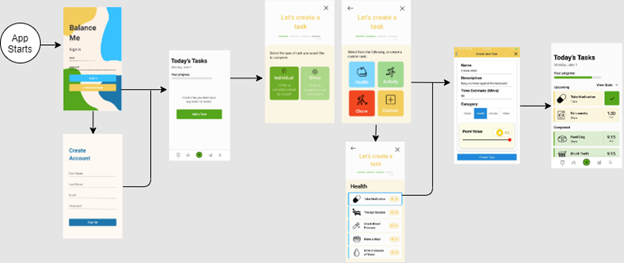
\includegraphics[width=1.0\columnwidth]{figures/flow}
%  \caption{The flow of screens the the user sees when creating a task in the
%	\textit{BalanceMe} mobile app. }~\label{fig:figure1}
%\end{figure}

With basic needs in mind, \textit{BalanceMe} achieves the requirements that one
would expect from a task management app. To differentiate ourselves, we focused
on providing functionalities that would allow the user to create, start and
finish a task with ease. To create a task, a user goes through a series of
screens that guide the user in creating the task (see Figure 1). Each screen
provides the user with 2-4 options that will decide what type of task will be
created. These options are presented as large colorful buttons that are light
on text. For re-usability purposes, a custom task created by users will be
saved in the local storage as part of the category tasks list. Currently, the
application only supports individual tasks. To aid the user in performing the
task, the user can add steps to the task during the creation process. These
steps will be displayed when the user starts the task. The user can also decide
to start the task now or schedule it for a later date.

For simplicity, tasks scheduled for within the 24 hours of the current day will
be displayed on the ``My Tasks'' screen.  From here, the user can either choose
to quickly complete a task or dive into a more guided step-by-step view by
clicking the task. On the ``My Tasks'' screen, each task is listed under one of
the four statuses: upcoming, in progress, completed, and overdue or missed. For
a visual cue, each task is color-coded to represent one of the four statuses.
As a motivational game element, the user can currently earn points for task
completion. Each task is assigned a point value, and users can view how many
points they have accrued on the ``My Tasks'' page. This feature is part of a
larger effort to add game elements to the \textit{BalanceMe} app, which can be
improved upon in future work.

\subsection{Back-End Development}
Our goal for the back-end design was to create a RESTful API that had direct
communication with our database. To do this, we used Express, Node.js, and
Mongoose for our server communication. For our database, we are using MongoDB
Atlas, as it provides us a database with lenient reading/writing and plenty of
space to hold our data. Furthermore, we are using Heroku to host our back-end
repository, which lets us make calls to our API from any device.

The reason we chose to use Mongoose is its models. Mongoose models utilize
schemas to let us easily layout what data we want each object type to
encapsulate. For the \textit{BalanceMe} app, this is the creation of two main
object types: User and Task. The user model holds information about each
individual user’s data, such as their first name and their email (see Figure 2).

\begin{figure}
\centering
  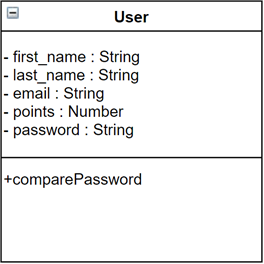
\includegraphics[width=0.6\columnwidth]{figures/user}
  \caption{A description of the User object type as it is stored in the
	\textit{BalanceMe} database. }~\label{fig:figure2}
\end{figure}

\begin{figure}
\centering
  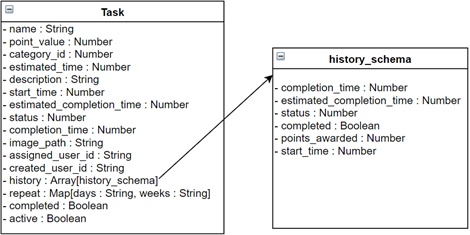
\includegraphics[width=1.0\columnwidth]{figures/task}
  \caption{A description of the Task object type as it is stored in the
	\textit{BalanceMe} database. }~\label{fig:figure3}
\end{figure}

In contrast to the simple user model, we created a task model that would be
capable of dynamic updates and easy repetition (see Figure 3).

Each task is referring to the user who created it and the user it is assigned
to. This allows for the possibility of another ``parent'' account to create a
task and assign it to a ``child'' account. This is outlined as a feature in the
in the \textit{Future Work} section of the document.

Another feature of our current implementation of the back-end is the creation
of local storage. We are using AsyncStorage to save a local user and local
default tasks. This allows us to have the user be automatically logged in when
they open the app and it allows for the use of quick default tasks for the user
to choose from. The local storage for the user’s information is directly synced
with the remote database. This allows the user to see their changes directly
and in real-time. The default task list is not directly synced with the remote
database, as we wanted each user’s default tasks to be individualized. This
creates a personalized list of both the original default tasks and the user’s
previously created tasks. We created the default task list so that task
creation could be quick and easy.

\subsection{Wearable Development}
Our companion application is a Fitbit smartwatch app. The goal of the companion
is to allow the user to be able to start and complete tasks from their watch,
and then sync up this data with the primary mobile app. We were able to complete
the first portion of this, and currently the user is allowed to select from a
preset list of tasks which they can then set a timer and complete, or set a
time to be completed later that day. The application has several screens,
starting with the list of preset tasks the user is allowed to choose from. Once
a task is selected, the user can then decide if they want to start the task
now or later. If the user chooses to start the task at the current time, a
timer screen is shown and the user can swipe to select the duration of the task
and the countdown will begin. If the user chooses to start the task at a later
time, they are taken to a screen that allows them to swipe up or down to select
a time. In the future, the smartwatch will vibrate or send a notification to
alert the user that it is time to complete the task.


\section{Discussion}

Reflecting back on our project, one of the most important learning outcomes
ended up being learning how to mix our initial goals with realistic outcomes.
At the midterm point in the project, we decided to re-evaluate our goals and
focus on the most important aspects and leave additional features to be added
in at the end if time permitted. This meant that instead of rushing to get
everything done, we instead placed an emphasis on quality over quantity. For
quantity, there were several parts of our original design, such as the
gamification and statistics screens, that we decided to leave out; they
didn’t fall in line as closely with the original aims of our project and we
realized we would not be able to complete them to the best of our ability
given the time constraints. To place an emphasis on quality, we decided to do
extensive testing and made smaller, minor improvements to improve the quality
of the app instead of major new features that were not guaranteed to be
completed on time.

Many of our group meetings revolved around this, and our project meetings
started to more resemble those in real-world software development companies. We
developed one week sprint cycles and created a priority list to sort through
the most important aspects of the application that needed to be completed in
order to provide a quality application to our end users. By the end of the
project, we were able to narrow the list to small bug fixes to improve existing
mobile and smartwatch screens, and the list was completed in the final week of
production. 

This shift in thinking and implementation offered an interesting learning
opportunity. As enthusiastic software developers, we all enjoyed brainstorming
and coming up with exciting and large new features to make our application
incredible. So, this decision to shift gears and slow down on the development
of major features and instead focus on minor improvements was a major change,
but we realized it was also still exciting and more akin to real world
production development. We ended up happier with the final product as a result,
which allowed us to create a quality product that demonstrated our hard work
and commitment to the project.


\section{Future Work}

%\begin{myitemize}
%  \setlength{\itemsep}{0pt}
%  \setlength{\parskip}{0pt}
%  \setlength{\parsep}{0pt}

While we accomplished a great deal over the course of this project, there is
still much more that can be done to improve the functionality and overall user
experience of \textit{BalanceMe}. These improvements are divided into three
larger categories: gamification and socialization, wearable expansion, and
general usability.

\subsection{Gamification and Socialization}

When we began work on this project, we set out to encourage users to complete
tasks by incorporating game elements into the app. In its current state,
\textit{BalanceMe} includes the ability to assign point values to each task,
and users can keep track of how many points they have earned via a progress bar
on the task list page. While this is a great foundation of a gamified task app,
future work could expand even further on this. Given more time, we would have
liked to include an avatar of the user’s choice as well as a progress tracking
dynamic graphic, such as a mountain with a climber that gets closer to the peak
the more points are earned. In addition to this, a reward could be given to the
user for reaching certain point goals. Rewards that were considered for this
feature included allotted relaxation time, virtual items like new avatars and
dynamic graphics, and custom rewards as dictated by the user’s parent or
guardian.

This heavier emphasis on game elements would go hand in hand with added
socialization features, including social media integration and designated
parent/guardian accounts. Ideally, the user would be able to connect
\textit{BalanceMe} to their Facebook or Twitter accounts and would then be able
to automatically post to their feeds whenever they accomplish a point milestone
goal. Additionally, \textit{BalanceMe} would be able to search the user’s
social media friends lists to find friends who have BalanceMe accounts. Users
would be able to compete with their BalanceMe friends to see who could score
the most points each week, adding yet another motivational game element to the
app.

The ability to connect with other \textit{BalanceMe} users would be a necessary
step to incorporate parent accounts into the app. Once implemented, a parent
account would have pseudo-admin privileges over their child’s \textit{BalanceMe}
account. This means that the parent or guardian could assign their child tasks
and keep an eye on their progress, all on their own mobile device. This feature
would be incredibly useful for parents of children with and without IDD.

\subsection{Wearable Expansion}
In its current state, the \textit{BalanceMe} Fitbit application has much less
functionality than the mobile application, which is how we planned it to be;
the Fitbit app should serve as a companion to the mobile app, with the Fitbit
providing richer functionality to the mobile experience instead of an
experience of its own. To that end, there is still more to be done on the
Fitbit side, namely implementing context awareness and cross-device
synchronization.

Our original idea for incorporating the wearable application into the
\textit{BalanceMe} project was to use its onboard sensors to provide real-time
context of a user’s actions. GPS and accelerometer data could be used to
determine a user’s location and intensity of motion, and microphones or light
sensors could provide even more contextual data. For example, if the app sees
that the user is mostly stationary (via accelerometer data) and has a task due
in 15 minutes, it would be able to send a reminder to the user to get up and
complete the task. This context awareness would be a cornerstone of
\textit{BalanceMe}’s functionality and is a great example of the usefulness of
ubiquitous computing.

To get this function to work properly, we would need to complete the
cross-device synchronization feature between the Fitbit and the mobile device.
Ideally, the user would be able to start a task on their Fitbit device using
the quickstart menu and then mark it as completed on their mobile app. This
feature would make using \textit{BalanceMe} much more convenient for the user.

\subsection{General Usability}
Further enhancements to the \textit{BalanceMe} experience include adding
cross-device system-level notifications for upcoming and in progress tasks,
scheduling conflict error handling, the ability to change the profile picture
and user password, and adding colors to the navigation tab bar on the mobile
app. The most important addition in this category would be to add a statistics
page where the user could see their task success and failures over time. This
data would be helpful for the user to analyze their task completion habits and
make meaningful changes to their routines.


\section{Conclusion}

With the development of \textit{Balance Me} we hope to create a product that
can help teenagers with and without IDD balance their time between required
tasks and leisure activities. We believe that the work that has been
accomplished so far is promising and will lead to an innovative solution for
this problem space. We believe that, by the end of the semester, we will have a
functioning product that enables users to improve their lives by successfully
managing their time.

\section{References}
[1] ``What is Intellectual Disability?'', \textit{SpecialOlympics.org}, 2020. [Online]. Available: https://www.specialolympics.org/about/intellectual-disabilities/what-is-intellectual-disability. [Accessed: 08- Jun- 2020].

[2] ``Focus Keeper - Time Management'', \textit{App Store}, 2020. [Online]. Available: https://apps.apple.com/us/app/focus-keeper-time-management/id867374917. [Accessed: 08- Jun- 2020].

[3] ``Toggl - Features'', \textit{Toggl.com}, 2020. [Online]. Available: https://www.toggl.com/
features/. [Accessed: 08- Jun- 2020].

[4] ``Stepping Stones - Daily Routines | Social App Hub'', \textit{Socialapphub.com}, 2020. [Online]. Available: https://www.socialapphub.com/app/stepping-stones-daily-routines. [Accessed: 08- Jun- 2020].

[5] ``CanPlan - a task manager app'', \textit{https://www.canassist.ca}, 2020. [Online]. Available: https://www.canassist.ca/EN/main/programs/technologies-and-devices/at-home/canplan.html. [Accessed: 08- Jun- 2020].

[6] ``A Task Timer for Special Education'', \textit{Resna.org}, 2020. [Online]. Available: https://www.resna.org/sites/default/files/legacy/conference/
proceedings/2003/Papers/TSP/Oleson\_TSP.htm. [Accessed: 08- Jun- 2020].

[7] ``Time Management | monday.com'', \textit{monday.com}, 2020. [Online]. Available: https://monday.com/lp/aw/timemgmt/remote. [Accessed: 08- Jun- 2020].

\end{document}